\section{Computational methods and theory}
\label{sec:methods}

\subsection{Background}
\label{sec:background}

Mixture models allow the expression of relatively complex marginal distributions
  fitting the observed variables in terms of more tractable joint
  distributions over the expanded space of observed and latent variables
  \citep{bishop_pattern_2009}.
The latent variables behave as simpler components used for building
  the inferred distribution from the observed data.
This general statistical framework provides not only the possibility
  of modeling complex distributions, % (e.g. \autoref{fig:model_fitted}),
  but also enables data to be clustered, using Bayes' theorem.
Given the generation and reconstruction processes involved in brain
  \gls*{mri}, it is accepted that these latent variables (the tissue
  classes) are reasonably well modeled with normal distributions
  \citep{van_leemput_automated_1999-1}.
Nonetheless, the existence of other minor sources of tissue contrast
  and the non-normality of several tissues under some conditions is
  widely accepted.
For instance, the \gls*{csf} is usually modeled with more than one
  normal distribution \citep{van_leemput_automated_1999-1,
  ashburner_unified_2005} to overcome these drawbacks.

A second relevant assumption is that the multivariate
  distributions associated with each expected cluster do
  not significantly overlap.
In the case of \gls*{mri} data, there are two principal sources of
  overlap in the observed tissue distribution: the \gls*{pv} effect and
  the \emph{bias field}.
On one hand, the so-called \gls*{pv} effect is remarkably related to
  tomographic biomedical imaging. Given that the images are defined
  on a grid of volume elements (voxels), they enclose a finite region.
This region may contain a mixture of signals from several
  tissues, producing an overlap between the tails of their distributions
  that can make the problem intractable by means of a
  \gls*{multivariate_gaussian}.
The number of voxels affected by the \gls*{pv} effect within a typical
  \gls*{mri} volume is usually significant, and worse when the resolution
  is low \citep{bromiley_multi-dimensional_2008}.
Previous studies have dealt with \gls*{pv} using non-normal intensity distribution
  models for each tissue \citep{santago_statistical_1995,noe_partial_2001,
  tohka_fast_2004}, modeling each cluster with more than one normal distribution
  \citep{ashburner_unified_2005,cuadra_comparison_2005},
  modeling the \gls*{mri} relaxation times at \gls*{pv}-affected voxels
  \citep{duche_bi-exponential_2012}, or
  using models with continuous latent variables \citep{liang_em_2009}.

On the other hand, most imaging datasets are affected to some degree
  by a spatially smooth offset field (called \emph{bias field}).
In \gls*{mri}, this illumination artifact derives from the spatial
  inhomogeneity of the magnetic field inside the scanner during
  acquisition.
Some retrospective techniques for tackling the bias field have
  been proposed, either embedded within the model
  \citep{van_leemput_automated_1999} or as a
  preliminary process \citep{tustison_n4itk:_2010}.

Finally, as \glspl*{multivariate_gaussian} are very sensitive to
  noise.
It is possible to introduce piecewise smoothness including
  spatial information in the described model, often
  implemented as a \gls*{markov}.
  
\subsection{Distribution model}
\label{sec:model}

\paragraph{\Acrlong*{multivariate_gaussian}}
Let $Y = \{\vy_i \in \mathbb{R}^C \}$ be a random variable that
  represents the observed data. Therefore, the image $Y$ is a stack
  of $C$ different \gls*{mri} sequences, and $i \in [1,\ldots,N]$
  is the index of each voxel in this image of $N$ voxels.
Accordingly, segmentation aims to obtain a certain realization of
  the latent random variable $X = \{ x_i \}$.
Thus, $Y$ is segmented after finding the class identified by 
  $l_k$ in the set of $K$ different clusters 
  $\mathcal{L} = \{l_1, l_2, \ldots, l_K \}$ that best matches
  $\vy_i$ given the model.
Finally, the \gls*{multivariate_gaussian} model is defined by two
  probabilities.
The first is the estimated normal distribution of each
  cluster, $\mathcal{N}(\vy_i \mid \theta_k )$, with
  $\theta_k = \{\boldsymbol{\mu}_k,\boldsymbol{\Sigma}_k\}$
  the parameters (means vector and covariance matrix)
  corresponding to the tissue identified by label $l_k$.
The second is the \emph{prior} probability of every voxel $i$
  belonging to cluster $l_k$, represented by $\pi_{k,i}$.

Using Bayes' theorem and the multivariate normal distribution as
  starting points, segmentation relies on iteratively improving the
  fitness of the model to the data.
To this end, \emph{posterior density} or \emph{responsibility} maps
  can be computed to evaluate the fitness \citep{bishop_pattern_2009}
  using the following expression:
\begin{equation}
\label{eq:post_density}
\gamma_{k,i}=P(x_i = l_k \mid \vy_i) = \frac
{\pi_{k,i} \, \mathcal{N}(\vy_i \mid \theta_k )}
{\sum_{j\in K} \pi_{j,i} \, \mathcal{N}(\vy_i \mid \theta_j ) },
\end{equation}
where $\gamma_{k,i}$ is the \emph{posterior density} of tissue class 
  $k$ at voxel $i$. Equivalently, $\gamma_{k,i}$ is the probability of
  detecting the class $l_k$ at $i$, given that $\vy_i$ was observed
  and the current model defined by $\lbrace \pi_{k,i}, \theta_k \rbrace$.
  
Once a stopping criterion has been met, the \emph{fuzzy} segmentation
  outcome is the set of \glspl*{tpm} corresponding to the last $\gamma_{k,i}$
  estimated, and the \emph{hard} segmentation $X$ is obtained after
  applying the \gls*{map} rule:
\begin{equation}
\label{eq:map}
\tilde{x}_i = \underset{\mathcal{L}}{\textrm{argmax}} \lbrace \gamma_{k,i} \rbrace
\end{equation}


\paragraph{Correction for bias field}
\label{sec:bias_model}
Let $B = \lbrace \vec{b}_i \in \mathbb{R}^C \rbrace$ be the unknown bias field,
  with $C$ independent components (one per input \gls*{mri} sequence).
It is a widely accepted assumption to consider $B$ a multiplicative smooth
  function of the pixel position \citep{vovk_review_2007}. Thus,
  we introduce this new random variable on the definition of the observation
  $\vy_i = \hat{\vy}_i \cdot \vec{b}^{T}_i$, where $\hat{\vy}_i$
  is the bias-free feature vector in $i$.
  
In order to extract $\hat{\vy}_i$, the observed variables $\vy_{i}$
  are logarithm transformed, so that $B$ becomes an additive field.
Thus, $B$ can be estimated by fitting a smooth function that minimizes
  the error field $E = \lbrace \vec{e}_i \rbrace$:
\begin{equation}
\label{eq:bias_error}
\vec{e}_{i} = \log{\hat{\vy}_{i}} - \log{\sum_{k\in K} \gamma_{k,i}\,\boldsymbol{\mu}_{k}}.
\end{equation} %

In \autoref{sec:em}, we shall discuss how to introduce the minimization
  of $E$ into the optimization routine for the estimation of $B$.
  
\paragraph{Regularization}
\label{sec:hmrf}
Finally, spatial constraints are included within the model in
  order to obtain a piece-wise smooth and plausible segmentation.
Typically, \gls*{multivariate_gaussian} methods are combined with the
  \gls*{markov} model to introduce such regularization.
The origin of \glspl*{markov} theory is the Gibbs distribution
  \citep{geman_stochastic_1984}, which has been comprehensively
  covered in the literature \citep{li_markov_2009}.
The spatial constraints are induced in the model throughout the 
  \emph{proportion factors} $\pi_{k,i}$ \eqref{eq:post_density}.
Therefore, assuming an \gls*{markov} model, $\pi_{k,i}$ now varies
  depending on the tissues located at the neighboring sites of $i$,
  the so-called \emph{clique} $\mathcal{N}_{i}$,
  with $i \notin \mathcal{N}_{i}$ and
  $i \in \mathcal{N}_{j} \iff j \in \mathcal{N}_{i}$.
\begin{equation}
\label{eq:hmrf_energy}
\pi_{k,i} \propto e^{\left(V_{i}(x_{i}=l_k)+\frac{\lambda_{\mathcal{N}}}{2}\underset{j\in\mathcal{N}_{i}}{\sum}V_{ij}(x_{i}=l_k,x_{j})\right)},
\end{equation}
where $V_{i}(x_{i})$ is an external field that weights the relative
  importance of the different classes present in the image and $V_{ij}(x_{i},x_{j})$
  models the interactions between neighbors.
Generally, $V_{i}(x_{i})=0$ is set in order to use a simplified model.
A typical definition of $V_{ij}(x_{i},x_{j})$ follows Pott's model
  \citep{zhang_segmentation_2001}:
\begin{equation}
\label{eq:potts_model}
V_{ij}(x_{i},x_{j})=\delta(x_{i},x_{j})=\begin{cases}
1, & \textrm{if}\: x_{i}=x_{j}\\
0, & \textrm{otherwise}.
\end{cases}
\end{equation}

\subsection{Optimization}
\label{sec:optimization}
Typically, the most common optimization of the described model has been
  solved by the \gls*{e_m} algorithm.
With the inclusion of the \glspl*{markov} into the model, the problem
  turns out to be a combinational one, intractable with \gls*{e_m}.
Therefore, a second solver is usually required for optimization
  of the full model.
A number of algorithms have been proposed for this application 
  \citep{bishop_pattern_2009}, for instance \gls*{icm},
  \gls*{montecarlo} sampling, or \gls*{graph_cuts}.

\paragraph{\Acrlong*{e_m} algorithm}
\label{sec:em}
\Gls*{e_m} iteratively seeks local solutions that are
  constantly closer to the global one.
For further details, we refer the reader to a theory book
  \citep{bishop_pattern_2009}.
In \autoref{alg:e_m}, we describe a modified version including
  the bias model estimation.
The \gls*{e_m} algorithm requires a good initialization of
  $\lbrace \pi_{k,i}, \theta_k \rbrace$, as it is
  likely to get trapped in local minima.
Typical initialization strategies can be automated, as the k-means algorithm,
  or the application of prior knowledge using \glspl*{tpm} from an atlas
  to estimate the initial parameters.
In addition, manual initialization is possible, explicitly specifying the
  model parameters.


\paragraph{\Acrlong*{graph_cuts} optimization}
\label{sec:background_graph_cuts}
The standard optimization procedure is to approximate the solution
  with the \gls*{e_m} algorithm and then impose the \gls*{markov}
  implicit regularization, as depicted in \autoref{fig:em_flowchart}.
The problem is stated so that we seek the labeling $X$ 
  that minimizes the following energy functional \citep{boykov_fast_2001}:
\begin{equation}
\Phi(X,Y)=\Phi_{smooth}(X)+\Phi_{data}(X,Y)
\label{eq:gc_energy}
\end{equation}
where $\Phi_{smooth}$ reflects the extent to which $X$ is not
  piecewise smooth, while $\Phi_{data}$ measures the 
  disagreement between $X$ and the observed data $Y$.

\Gls*{graph_cuts} algorithms approximately minimize the energy $\Phi(X,Y)$
  for the arbitrary finite set of labels $\mathcal{L}$ under two fairly
  general classes of interaction penalty $V_{ij}$:
  \emph{metric} and \emph{semi-metric} \citep{boykov_fast_2001}.
In the case of $n=2$ this solution is exact, as opposed to greedy algorithms
  like the widely used \gls*{icm}.
Weighted graphs encoding all possible energy configurations
  are built as follows.
The nodes of the graph are the two possible labels and each voxel of
  the image grid.
All nodes corresponding to image voxels are linked to the nodes
  of the labels, encoding on the edge weight the membership likelihood.
Edges between voxel nodes encode the pair-wise interactions of the
  \gls*{markov} system.
The minimum of the energy functional \eqref{eq:gc_energy} concurs on 
  the minimum cut of the graph.
In graph theory, a cut is a partition of the vertices of the graph
  in disjoint subsets.
The size of a cut depends on the number and weights of the edges
  removed.
Therefore, the minimum cut is that not larger than the size of any
  other cut.
  
The binary case is extended to $n$-cluster classification
  with iterative algorithms of very large binary \emph{moves}
  (a simultaneous and large change of assigned labels in $X$).
The basic underlying concept is to find local minima sequentially
  at each iteration, based on the allowed moves.
\citeauthor{boykov_fast_2001} \citep{boykov_fast_2001,kolmogorov_what_2004}
  proposed two different algorithms to implement \gls*{graph_cuts},
  called $\alpha$-expansion and $\alpha\beta$-swap.
In \autoref{alg:swap} (Appendix B), we describe $\alpha\beta$-swap to illustrate
  how the iterative minimization works.
Both algorithms have been proven to be highly accurate and efficient
  approximations of the global minimum for $n$-cluster classification
  \citep{boykov_experimental_2004}.
  
\subsection{Implemented methods and contributions}
\label{sec:implementation_details}
\Gls*{mbis} implements the general \gls*{multivariate_gaussian} model as
  described in \autoref{sec:model}.
We specify in this section the main contributions and features
  implemented in \gls*{mbis}.
An overview of the principal elements of the tool and the optimization
  strategy is presented in \autoref{fig:em_flowchart}.
\begin{figure*}[t]
	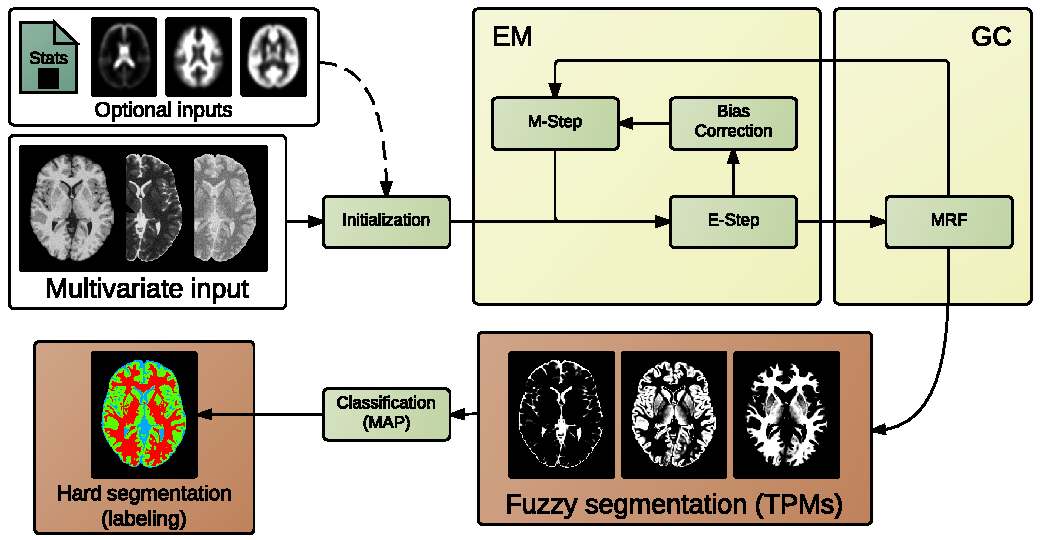
\includegraphics[width=1.0\linewidth]{fig01-generic-flowchart}
	\caption[Segmentation flowchart]{\Gls*{e_m}-\gls*{graph_cuts} segmentation
	takes as inputs the blocks depicted in white background and produces the
	blocks in brown background as outputs.
	Typically, the initialization can be performed supplying a file with
	the parameters of the model, or prior \glspl*{tpm} from an atlas (optional
	inputs are represented with a dashed line connector).}
	\label{fig:em_flowchart}
\end{figure*}

\paragraph{Initialization}\label{par:initialization} %
Once the model has been fully defined (number of expected pure tissues,
  number of normal distributions per tissue, number of special \gls*{pv}
  classes, and bias correction), \gls*{mbis} allows
  for several standard initialization approaches.
One common and fully-automated strategy is the use of the
  k-means algorithm, which is the default option in \gls*{mbis} when
  no other initialization is required.
A second extended initialization strategy is manually setting $\{\theta_k\}$,
  assuming a uniform distribution for $\pi_{k,i}$.
Finally, it is also common to use atlas priors when the spatial mapping
  between the actual case and the atlas is known.
Atlas priors can be supplied to \gls*{mbis} as a set of \glspl*{tpm},
  one per normal distribution.
It is important to note that these priors are no longer applied
  after initialization.

\paragraph{Bias correction}\label{par:bias_correction} %
When bias correction is required, a new definition of likelihood
  derived from \eqref{eq:post_density} is applied.
We estimate the bias field $B$ approximating the error measurement map
  $E$ obtained after \eqref{eq:bias_error} with uniform B-splines.
This solution is dual to N4ITK, the non-parametric algorithm presented
  elsewhere \cite{tustison_n4itk:_2010}.
\citeauthor{tustison_n4itk:_2010} analyzed the best B-spline parametrization
  for bias correction, and concluded that it is preferable to other models
  based on linear combinations of polynomial or smooth basis functions.
Before the next iteration of the E-step (see \autoref{alg:e_m}), data are
  corrected with the field vector $\vec{b}_{i}$ at $i$ before the distribution 
  parameters are calculated.

\paragraph{\Acrlong*{pv} model}\label{par:model} %
On the basis of previous findings \citep{cuadra_comparison_2005}, \gls*{mbis}
  tackles the \gls*{pv} effect by modeling pure tissues with \emph{in-class}
  mixtures of normal distributions, and by adding specific \gls*{pv} classes
  \citep{noe_partial_2001}.
Appropriate transition penalties can be set consistently for these classes, as
  in \citep{cuadra_comparison_2005}.
Instead of estimating the tissue contributions to the \gls*{pv} classes
  within the model, we provide a simplified procedure to achieve this aim
  \emph{a posteriori}.
The methodology computes the Mahalanobis distance \eqref{eq:mahalanobis}
  of the \gls*{pv} samples to the tentative pure tissues.
Interpreting the posterior probability as a volume fraction of the tissue
  within the voxel, this volume is divided between the pure tissues inversely
  proportional to the distance $D_k$ \eqref{eq:mahalanobis} to the tissues.
This \gls*{pv} solving is applied to the experimental results presented
  in \autoref{sec:results}.
\begin{equation}
\label{eq:mahalanobis}
D_k(\vy_i) = \sqrt{(\vy_{i}-\boldsymbol{\mu}_{k})^{T}\boldsymbol{\Sigma}_{k}^{-1}(\vy_{i}-\boldsymbol{\mu}_{k})}.
\end{equation}

\paragraph{\Acrlong*{graph_cuts} optimization}\label{par:graphcuts_optimization} %
\Gls*{mbis} implements \gls*{graph_cuts} optimization as in \citep{boykov_fast_2001},
  wrapping the \emph{maxflow} library (\url{http://vision.csd.uwo.ca/code/})
  in \gls*{itk} to solve the graphs.
The weighting parameter $\lambda_{\mathcal{N}}$ \eqref{eq:hmrf_energy} must be
  adequately determined for sensible regularization.
In \autoref{sec:brainweb_evaluation}, we describe the experiment conducted to
  set $\lambda_{\mathcal{N}}$ empirically.
The special \gls*{pv} classes are taken into account specifying an appropriate
  transition model.
The transition model is a matrix where the interactions between individual normal
  distributions are defined.
These energy interactions are defined by the $V_{ij}(x_{i},x_{j})$ presented in
  \autoref{sec:hmrf}.
Generally, in an \gls*{markov} model including several normals distributions per
  tissue (to account for \gls*{pv} effects), transitions within pure tissue have
  lower penalties (inner transitions) than transitions between pure tissues
  (outer transitions).
\Gls*{mbis} supports complex neighboring systems (beyond the simplest Pott's model
  \eqref{eq:potts_model}), distance weighted energy interactions, and non-metric
  tissue transition models.